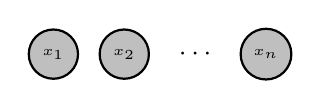
\begin{tikzpicture}[scale=0.3] % , baseline = -3.5pt


	\node [circle, draw, thick, fill=gray!50] (T1) at (0,0) {\tiny $x_1$};
	\node [circle, draw, thick, fill=gray!50] (T2) at (3,0) {\tiny $x_2$};

\node[anchor=center] (text) at (6,0) {$\cdots$};

	\node [circle, draw, thick, fill=gray!50] (T3) at (9,0) {\tiny $x_n$};
	

\end{tikzpicture}